\documentclass[12pt]{article}
\usepackage[utf8]{inputenc}
\usepackage[top=0.75in, bottom=0.75in, left=0.75in, right=0.75in, headheight=15pt]{geometry}
\usepackage{amsmath, amssymb, amsthm, graphicx, hyperref, enumerate, multirow,  multicol, tikz, centernot, cancel, forest, lipsum, mathtools, bm, esvect, fancyhdr, esdiff, float, parskip, comment}

\DeclareMathSymbol{*}{\mathbin}{symbols}{"01} % change * to /cdot inside math
% \begingroup % let only this align, etc. break across pages
% \allowdisplaybreaks
% \begin{align}
%     ....
% \end{align}
% \endgroup

% \texorpdfstring{$k$}{k} math inside (sub/)section label

\pagestyle{fancy}
\fancyhead[L]{Liheng Cao}
% \fancyhead[C]{center}
\fancyhead[R]{}

\title{ML Homework 4}
\author{Liheng Cao}
% \date{Date}

\begin{document}
\maketitle

\section{}
When $ w_0 $ increases, then the probability of predicting class 1 becomes higher, and vice versa. 
\[ h(x) = \dfrac{1}{1+e^{-(w_0 + \cdots)}} \]
This is because as $ w_0 $ gets bigger, the result of exponentiation gets smaller. As the denominator gets smaller, the quotient gets larger. $ h(x) $ is used as the probability we will predict a certain class. The higher $ h(x) $ is, the more likely we will predict class 1 (as opposed to class 0).
\newpage

\section{}
The logistic function is \[ \dfrac{1}{1+e^{-\textbf{w}^T \textbf{x}}} \]
If we were to double $ \textbf{w} $, the result wouldn't actually change, as long as the threshold is 0.5. 

The geometric interpretation is because $ \textbf{w}^T\textbf{x} $ represents a (hyper)plane. Multiplying the equation of a plane doesn't affect any points that are on the plane (threshold = 0.5 $\implies$ on hyperplane), but it makes the points that are off it seem further away, increasing the certainty with which we pick a class. For example, if $ \textbf{w}^T\textbf{x} = 0$, then there is no change ($ 0 * 2 = 0 $). But if it's positive, it becomes a larger positive number, and vice versa.
\newpage

\section{}
\begin{enumerate}[(a)]
	\item 
	\[\begin{bmatrix}
		3 & 1 \\
		1 & 3 \\
	\end{bmatrix}\]
	
	\item 
	\begin{figure}[H]
	    \centering
	    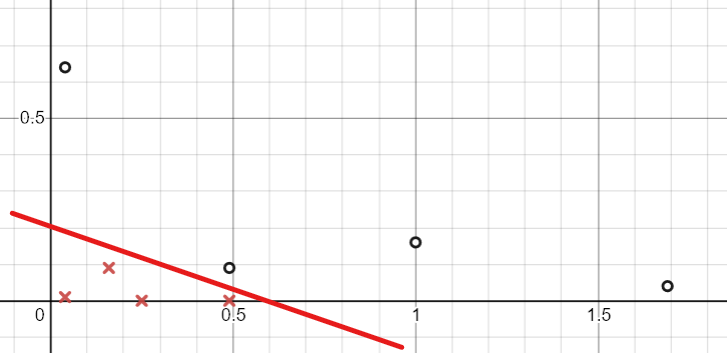
\includegraphics{assignments/intro to ml/ml hw4/images/3b.png}
	    \caption{o: class 0, x: class 1}
	    \label{fig:3:b}
	\end{figure}
\end{enumerate}


\end{document}